\section{Water and cabbages in $\mathbb{F}_1$-geometry}
Today we'll try to grasp the meaning of Chebotar\"ev's density theorem, and hint at how this may help us get a fix on~$\mathbb{F}_{1}$-geometry, formerly known as recreational number theory.

\subsection{Status quo}

In our weekly seminar the problem at hand is to classify the~$\mathbb{F}_{1}$-subschemes of~$\mathbb{P}^{1}_{\mathbb{Z}}=\mathbb{P}^{1}_{\mathbb{F}_{1}}\times_{\mathbb{F}_{1}}\mathrm{Spec}(\mathbb{Z})$. This boils down to finding the ordinary~$\mathbb{Z}$-subschemes that also carry a~$\lambda$-structure. Solving this problem will help us formalize Smirnov's approach to~$\mathbb{F}_{1}$-geometry, as put forward in~\cite{hurwitz-inequalities-for-number-fields}. To do so, crucial tools will be provided for by several density theorems in algebraic number theory. My experience in number theory is almost nonexistent, so it seems like a good idea to conjure up a post on the subject, with a little help from (once again) Hendrik Lenstra, in~\cite{chebotarev-and-his-density-theorem}.

\subsection{Chebo-who?}

\begin{wrapfigure}[14]{r}{.35\textwidth}
  \centering
  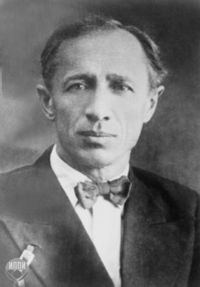
\includegraphics[width=.3\textwidth]{chebotarev-density/chebotarev}
  \caption{Nikol\"ai Chebotarev}
\end{wrapfigure}

Nikola\"i Chebotar\"ev (1894--1947) was a Russian number-theorist, famous for his proof of a conjecture by Frobenius. The conjecture had been open for 42 years before Cheb tamed it, and surprisingly (at least to me) it provided just the right ingredient for Artin to prove his well-known reciprocity law, vastly generalizing the baby version put forward by Gauss, as in Section~\ref{advanced-alchemy}. In fact, if Artin had waited a while longer to publish his paper, chances would have been in favour of the less groovy sounding Chebotar\"ev reciprocity. If you're stuck for inspiration, let me just mention that Nikola\"i (shown here with an exquisite bowtie) didn't like working at a desk, but preferred a comfy bed to get the job done.

\subsection{Densely packed}

To explain the theorem, it'll be worthwhile to check out the cases it generalizes: Dirichlet's theorem on primes in arithmetic progressions, and Frobenius density. Very naturally, a set of primes~$S$ is said to have density~$\delta$ if the ratio of the number of primes in~$S$, smaller than a number~$n$, to the number of all primes smaller than~$n$ converges to~$\delta$, for~$n \to \infty$. The Dirichlet theorem then says

\begin{theorem}
  Fix~$m \in \mathbb{Z}$. If an arbitary integer~$a$ is coprime with~$m$, then the set of primes~$p$, with~$p \equiv a\bmod m$, has density~$1/\varphi(m)$,~$\varphi$ being Euler's totient function.
\end{theorem}

Specializing to the case~$m=10$, you get the intuitive result that there are ``as many'' primes ending in~$1$, as there are in~$3, 7$ and~$9$ respectively.

\subsection{Frobenius' highest honour}

Frobenius, the only mathematician I know of who's also a noun, has his own density theorem. To formulate it correcty, we need two new concepts, decomposition type and cycle pattern. Given a monic integer polynomial of degree~$d$ with non-zero discriminant~$\Delta(f)$, and a prime~$p$ that doesn't divide~$\Delta(f)$, you can factor~$f\bmod p$ into~$n$ distinct irreducibles. The numbers $d_{1},\ldots,d_{n}$, with~$d_{i}$ the degree of the~$i$-th factor in this decomposition, comprise the decomposition type of~$f\bmod p$. Notice that the~$d_{i}$ form a partition of~$d$. Since~$f$ has~$d$ different roots~$\alpha_{1},\ldots,\alpha_{d}$, the Galois group~$G$ of~$f$ consists of~$\mathbb{Q}$-automorphisms of~$\mathbb{Q}(\alpha_{1},\ldots, \alpha_{d})$. Elementary Galois theory says this is a subgroup of~$S_{d}$, so every element~$\sigma \in G$ can be written as a product of disjoint cycles, including cycles of length~$1$. The length of each of these cycles will again form a partition of the degree~$d$, the cycle pattern. Frobenius connects the two.

\begin{theorem}
  The set of primes~$p$ for which~$f$ has a given decomposition type~$d_{1},\ldots,d_{n}$ has a density which is equal to~$1/\vert G \vert$ times the number of~$\sigma \in G$ with cycle pattern~$d_{1},\ldots,d_{n}$.
\end{theorem}

Considering a special case once again, look at the partition~$d=1+\ldots+1$. Trivially, only the identity has this as a cycle pattern, and thus we see that the number of primes~$p$ for which~$f$ splits into linear factors has density~$1/\vert G \vert$. It's worth noting that by using a good algebra program like GAP{,} you can use this result to determine the order of the Galois group of a polynomial, and a fortiori the group itself. If your gut feeling is that the two theorems are connected, you're absolutely right! To make this concrete, we'll need Chebotar\"ev's result.

\subsection{Chebo-what?}

In general, Dirichlet for a certain~$m$ implies Frobenius for the polynomial~$X^{m}-1$. To see this for the special decomposition type~$1,1,\ldots,1$, remember that the Galois group of~$X^{m}-1$ is isomorphic to the unit group of~$\mathbb{Z}/m\mathbb{Z}$, which has~$\varphi(m)$ elements. Taking~$a$ to be~$1$ in Dirichlet's theorem, we see that the set of primes for which~$p \equiv 1\bmod m$ is equal to the set of primes for which~$X^{m}-1$ splits into linear factors, by Fermat's little theorem. The general case is not much harder, but requires a couple of properties of finite fields I won't go into. The problem rests in the converse. Given the statement of Frobenius density, a first natural question to ask is whether we can always find for a given prime~$p$ that doesn't divide~$\Delta(f)$, an element~$\sigma_{p} \in G$, such that the decomposition type of~$f\bmod p$ equals the cycle pattern of~$\sigma_{p}$. This can be done up to conjugacy, which seems logical, since conjugate permutations also have the same cycle pattern. Chebotar\"ev's theorem then deals with the density of the set of those primes~$p$ for which~$\sigma_{p}$ is equal to a given element of~$G$.

It seems best to postpone the detailed formulation of Chebotar\"ev's theorem, since I need some more technical stuff like \emph{places}, which would make this post unnecessarily long. Let me finish by explaining the first part of the title with a quote from (tadaa) Lenstra:
\begin{quote}
  So, Chebotar\"ev had to carry water and cabbages from the lower part of Odessa to the higher part of Odessa. This is, of course, the most difficult direction.
\end{quote}
Inspite of its humorous simplicity, I can't stop thinking about this quote which, like most of Lenstra's \emph{debaucheries}, says more than meets the eye.
